\documentclass{protokol}
\usepackage{graphicx}
\usepackage{float}

\usepackage{tikz}
\usetikzlibrary{calc}
\usetikzlibrary{arrows}


%====== Units =====
\usepackage{amssymb}
\usepackage{siunitx}
\sisetup{inter-unit-product =\ensuremath{\cdot}}
\sisetup{group-digits = integer}
\sisetup{output-decimal-marker = {,}}
\sisetup{exponent-product = \ensuremath{\cdot}}
\sisetup{separate-uncertainty}
\sisetup{tight-spacing = false}
%\sisetup{scientific-notation = true}
%\sisetup{round-mode=places,round-precision=4}
%\sisetup{evaluate-expression}


%====== Grafy =====
\usepackage{pgfplots}
\pgfplotsset{width=0.8\linewidth, compat=1.17}
\def\plotcscale{0.8}
\usepackage{pgfplotstable}
\usepackage[figurename=Obr.]{caption} % figure caption rename

\usepackage[siunitx]{circuitikz} % obvody
% \ctikzset{bipoles/length=1cm}

%====== Rovnice align block ======
\usepackage{amsmath}
\setlength{\jot}{10pt} % rozestup mezi řádky

\graphicspath{ {./img/} }

%====== Code blocks ======
\usepackage{listings}

\usepackage[most]{tcolorbox}
\newtcbox{\inlinecode}{on line, boxsep=0pt, left=2pt, right=2pt, top=2pt, bottom=2pt, colframe=gray, boxrule=0.5pt, arc=1pt, auto outer arc, before upper={\vphantom{dlg}}, tcbox raise base} % vytvoření inline boxu pro kód

\lstdefinelanguage{Spice}{
    alsoletter={.},  % Přidává tečku jako součást slov
    morekeywords={.lib, .STEP, .param, .MEAS, FIND, WHEN, END, VALUE, R, C, L, K, .SUBCKT, .ENDS, .MODEL, .INCLUDE, .AC, .DC, .TRAN, .PRINT, .PLOT, .PROBE, .WIDTH, .OPTIONS, .NODESET, .IC},
    keywordstyle=\color{blue}\bfseries,
    sensitive=false, % klíčová slova nejsou citlivá na velikost písmen
    morecomment=[l]{;}, % komentáře začínají hvězdičkou
    morestring=[b]", % řetězce uzavřené do uvozovek
}

\lstset{
  language=Spice,
  basicstyle=\ttfamily\small,
  breaklines=true,
  numbers=left,
  numberstyle=\tiny\color{gray},
  frame=single,
  rulecolor=\color{black},
  title=\lstname,
  keywordstyle=\color{blue}\bfseries,
  commentstyle=\color{green},
  stringstyle=\color{red},
  showstringspaces=false
}

%====== Vyplňte údaje ======
\jmeno{Tomáš Vavrinec}
\kod{240893}
\rocnik{}
\obor{MET}
\skupina{}
\spolupracoval{--}

\merenodne{--}
\odevzdanodne{--}
\nazev{2. Zdroje referenčních proudů a napětí}
\cislo{3} %měřené úlohy

\predmet{Návrh analogových integrovaných obvodů}
\ustav{Ústav mikroelektroniky}
\skola{FEKT VUT v~Brně}

\def\para{x+0}
\def\parb{\para-80}


%citace 
\usepackage[backend=biber, style=iso-numeric, sortlocale=cs_CZ, autolang=other, language=czech]{biblatex}
\addbibresource{bibliography.bib}
\DeclareFieldFormat{labelnumberwidth}{\mkbibbrackets{#1}}
% hyperlinky
\usepackage[colorlinks]{hyperref}

% odstavce
\usepackage{parskip}

% Bloky kódu
\usepackage{xcolor}

%New colors defined below
\definecolor{codegreen}{rgb}{0,0.6,0}
\definecolor{codegray}{rgb}{0.5,0.5,0.5}
\definecolor{codepurple}{rgb}{0.58,0,0.82}
\definecolor{backcolour}{rgb}{0.95,0.95,0.92}

\usepackage{listings}
\lstdefinestyle{mystyle}{
  backgroundcolor=\color{backcolour}, commentstyle=\color{codegreen},
  keywordstyle=\color{magenta},
  numberstyle=\tiny\color{codegray},
  stringstyle=\color{codepurple},
  basicstyle=\ttfamily\footnotesize,
  breakatwhitespace=false,         
  breaklines=true,                 
  captionpos=b,                    
  keepspaces=true,                 
  numbers=left,                    
  numbersep=5pt,                  
  showspaces=false,                
  showstringspaces=false,
  showtabs=false,                  
  tabsize=2
}
\lstset{
	inputencoding=utf8,
	extendedchars=true,
	literate={á}{{\'a}}1 {č}{{\v{c}}}1 {ď}{{\v{d}}}1 {é}{{\'e}}1 {ě}{{\v{e}}}1 
           {í}{{\'i}}1 {ň}{{\v{n}}}1 {ó}{{\'o}}1 {ř}{{\v{r}}}1 {š}{{\v{s}}}1 
           {ť}{{\v{t}}}1 {ú}{{\'u}}1 {ů}{{\r{u}}}1 {ý}{{\'y}}1 {ž}{{\v{z}}}1 
           {Á}{{\'A}}1 {Č}{{\v{C}}}1 {Ď}{{\v{D}}}1 {É}{{\'E}}1 {Ě}{{\v{E}}}1 
           {Í}{{\'I}}1 {Ň}{{\v{N}}}1 {Ó}{{\'O}}1 {Ř}{{\v{R}}}1 {Š}{{\v{S}}}1 
           {Ť}{{\v{T}}}1 {Ú}{{\'U}}1 {Ů}{{\r{U}}}1 {Ý}{{\'Y}}1 {Ž}{{\v{Z}}}1,
	style=mystyle
	}

% Číslování
\pagenumbering{arabic}



% =========================================
% =============== DOKUMENT ================
% =========================================
\begin{document}
	%====== Vygenerování tabulky ======
	\maketitle

\section*{ZADÁNÍ ÚLOHY}
  Detailní popis jednotlivých úloh s návodem najdete v NAO\_PC.pdf, který je dostupný v E-learningu.

\begin{itemize}
    \item {\bf Simulací získejte hodnoty prahového napětí \(U_{TH0}\) pro dvě různé řady rozměrů tranzistorů.}
    \begin{itemize}
        \item konstantní poměr \(W/L = 5, kdy \$L\$ = 0.18; 0.3; 0.5; 0.8; 1; 2; 3; 5; 10\),
        \item různé rozměry: \(W/L = 0.22/0.18; 1/0.5; 2/0.5; 2/1; 5/1; 5/2; 10/5; 10/10; 40/10\),
        \item výše uvedené dva body budou provedeny pro tranzistor NMOS i PMOS.
    \end{itemize}
    \item {\bf Závislost prahového napětí \(U_{TH}\) na \(U_{SB}/U_{BS}\) (bulk efekt) Simulací získejte hodnoty prahového napětí \(U_{TH}\) pro napětí \(U_{BS}\) (NMOS) resp. \(U_{SB}\) (PMOS) v rozsahu \(0 [V]\) až \(500 [mV]\) s krokem \(50 [mV]\).}
    \item {\bf Závislost parametru modulace délky kanálu (\(\lambda\)) na délce kanálu (L) Simulací získejte hodnoty parametru \(\lambda\) tranzistoru NMOS a PMOS pro L v rozmezí \(200 [nm]\) až \(10 [\mu m]\).}
\end{itemize}

\subsection*{Bonusové otázky (1 b.)}
\begin{itemize}
    \item Popište, jak byste simulací (mimo analýzu \inlinecode{.op}) zjistili transkonduktanci \(gm\).
          Nakreslete schéma, popište nastavení a odečet hodnot.
\end{itemize}

\setcounter{section}{0}

\newpage
\section{Vypracování}
  \subsection{Proudová reference} 
  Jako první určíme rozměry použitých tranzistoru.
Volím délku kanálu \(L = 2 [\mu m]\) jako kompromis mezi velikostí a parametrem \(\lambda\), která pro \(L = 2 \mu m\) nabývá hodnoty \(\lambda = 0.0787698 [V^{-1}]\).
Dále musíme zvolit napětí \(U_{OV}\), které volím s ohledem na rozsah napájecího napětí \(U_{OV} = 0.2 [V]\)
Z toho následně můžeme určit šířku kanálu \(W\), tranzistorů \(M1\) a \(M3\) jako:

\begin{center}
    \large
    \(
        W_{M1} = W_{M3} = L \cdot \frac{2 \cdot I_1}{KP \cdot U_{OV}^2} = 2\mu \cdot \frac{2 \cdot 10\mu}{200\mu 0.2^2} = 5 [\mu m]
    \)
\end{center}

obdobně určíme rozměry tranzistorů \(M2\) a \(M4\) jako:

\begin{center}
    \large
    \(
        W_{M2} = W_{M4} = L \cdot \frac{2 \cdot I_1}{KP \cdot U_{OV}^2} = 2\mu \cdot \frac{2 \cdot 10\mu}{50\mu 0.2^2} = 20 [\mu m]
    \)
\end{center}

Z čehož snadno určíme \(W_{M6}\) jako:

\begin{center}
    \large
    \(
        W_{M6} = W_{M2} \cdot \frac{I_2}{I_1} = 20\mu \cdot \frac{50\mu}{10\mu} = 100 [\mu m]
    \)
\end{center}

\begin{center}
    \large
    \(
        r_1 = \frac{U_{TH-M1}+U_{OV-M1}}{I_1} = \frac{0.384+0.2}{10\mu} = 58.4 [k\Omega] 
    \)
\end{center}

\vspace{10mm}
\begin{figure}[h!]
    \centering
    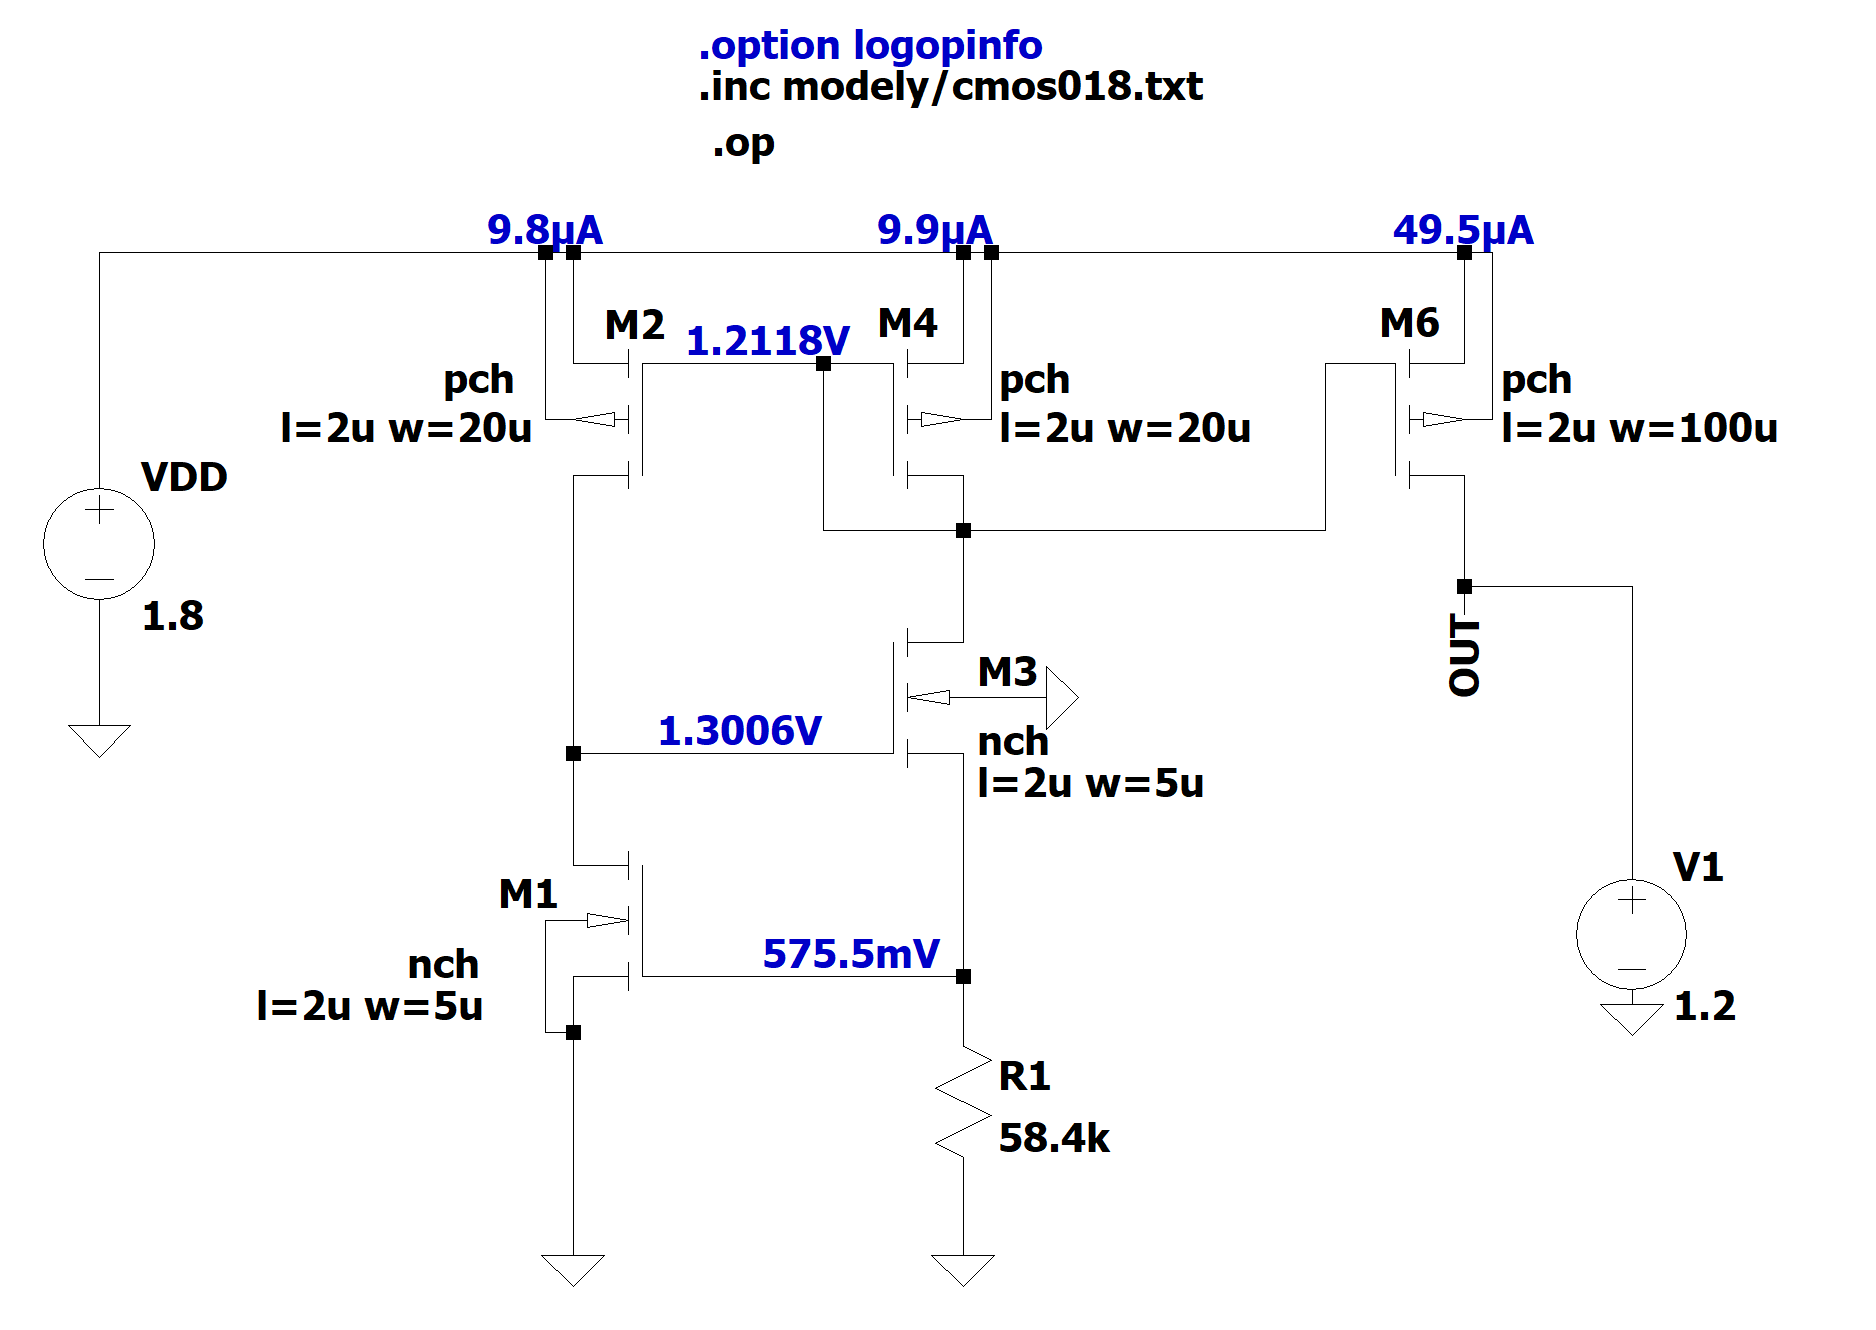
\includegraphics[width=0.9\textwidth]{text/img/PR-op-sch.png}
    \caption{\label{fig:KPZ-op-sch} Zobrazení napětí a proudu ve schématu}
\end{figure}

\vspace{10mm}
\begin{figure}[h!]
    \centering
    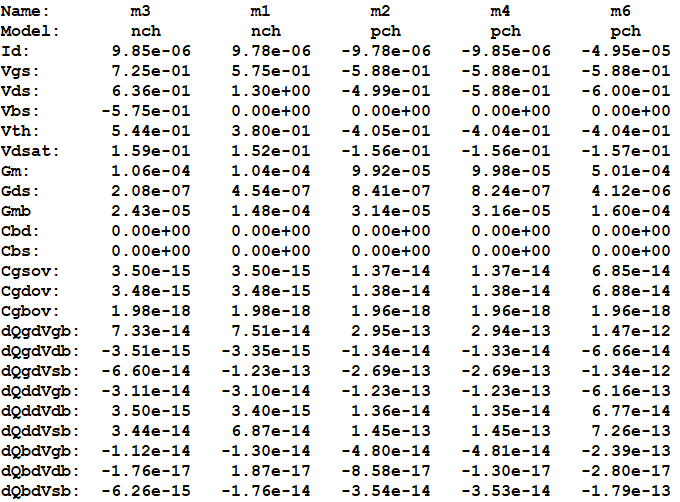
\includegraphics[width=0.9\textwidth]{text/img/PR-op-ol.png}
    \caption{\label{fig:KPZ-op-ol} Pracovní bod tranzistorů}
\end{figure}



  \newpage
  \clearpage

  \subsection{Napěťová reference} 
  Jako první určíme rozměry použitých tranzistoru.
Volím délku kanálu \(L = 2 [\mu m]\) jako kompromis mezi velikostí a parametrem \(\lambda\), která pro \(L = 2 \mu m\) nabývá hodnoty \(\lambda = 0.0787698 [V^{-1}]\).
Dále musíme zvolit napětí \(U_{OV}\), které volím \(U_{OV} = 0.5 [V]\) jelikož pracovní napětí mám jasně dané, větší pracovní rozsah tak nepotřebuji a radši použiji menší tranzistor.
Z toho následně můžeme určit šířku kanálu \(W\) jako:

\begin{center}
    \large
    \(
        W = L \cdot \frac{2 \cdot I_T}{KP \cdot U_{OV}^2} = 2\mu \cdot \frac{2 \cdot 40\mu}{200\mu 0.5^2} = 3.2 [\mu m]
    \)
\end{center}

Dále určíme společný odpor rezistorů \(r_2\) a \(r_3\) jako:

\begin{center}
    \large
    \(
        r_{2,3} = \frac{U_{OUT}}{I_1-I_2} = \frac{1.2}{50\mu - 50\mu} = 120 [k\Omega] 
    \)
\end{center}

Z čehož můžeme určit \(r_3\) jako:

\begin{center}
    \large
    \(
        r_3 = \frac{U_{TH}+U_{OV}}{U_{OUT}} \cdot r_{2,3} = \frac{0.384+0.5}{1.2} \cdot 120\cdot 10^{3} = 88.4 [k\Omega]
    \)
\end{center}

\(r_2\) pak určíme jednoduše jako:

\begin{center}
    \large
    \(
        r_2 = r_{2,3} - r_{3} = 120 \cdot 10^{3} - 88.4 \cdot 10^{3} = 31.6 [k\Omega]
    \)
\end{center}

Nakonec určíme odpor \(r_1\) jako:

\begin{center}
    \large
    \(
        r_1 = \frac{U_{CC}-U_{OUT}}{I_{1,2}} = \frac{1.8-1.2}{50\mu} = 12 [k\Omega] 
    \)
\end{center}

\vspace{10mm}
\begin{figure}[h!]
    \centering
    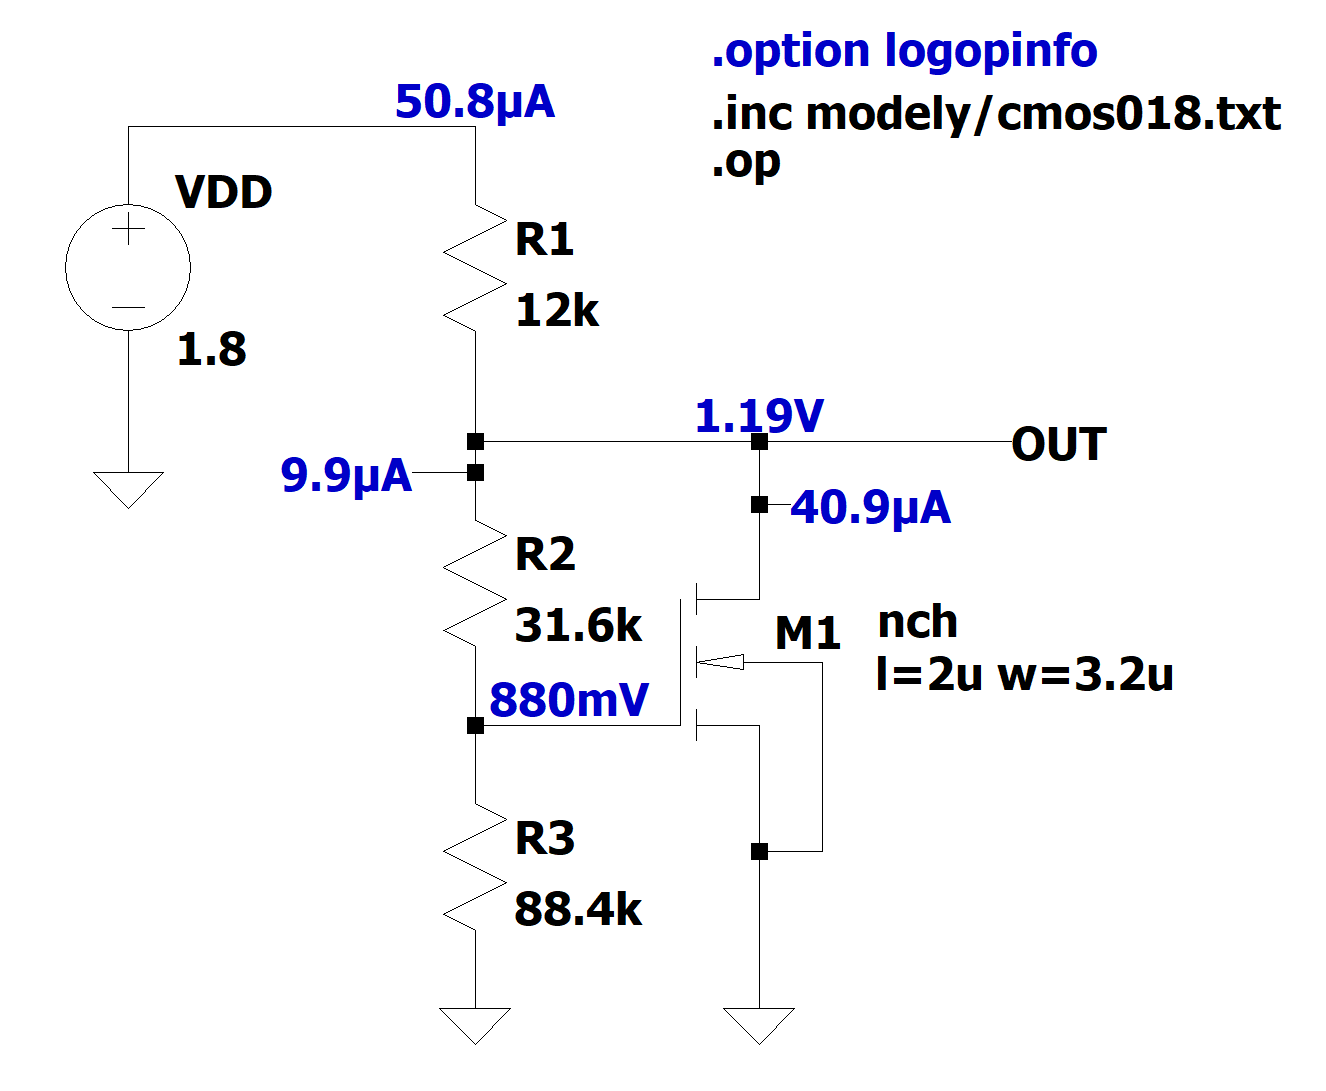
\includegraphics[width=0.9\textwidth]{text/img/NR-op-sch.png}
    \caption{\label{fig:NR-op-sch} Zobrazení napětí a proudu ve schématu}
\end{figure}

\vspace{10mm}
\begin{figure}[h!]
    \centering
    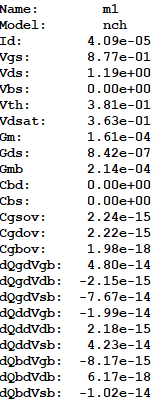
\includegraphics[width=0.3\textwidth]{text/img/NR-op-ol.png}
    \caption{\label{fig:NR-op-ol} Pracovní bod tranzistoru}
\end{figure}


  \newpage

  \subsection{Napěťová reference s proudovým zdrojem} 
  V předchozím příkladě napěťové reference sloužil odpor \(r_1\) jako proudoví zdroj.
Protože jde jen o rezistor nebude to dvakrát přesný proudoví zdroj a proto ho nyní nahradíme proudovým zdrojem z předcházejícího příkladu.
Hodnoty všech prvku zůstávají zachovány a výsledkem je tedy následující schéma.

\begin{figure}[h!]
    \centering
    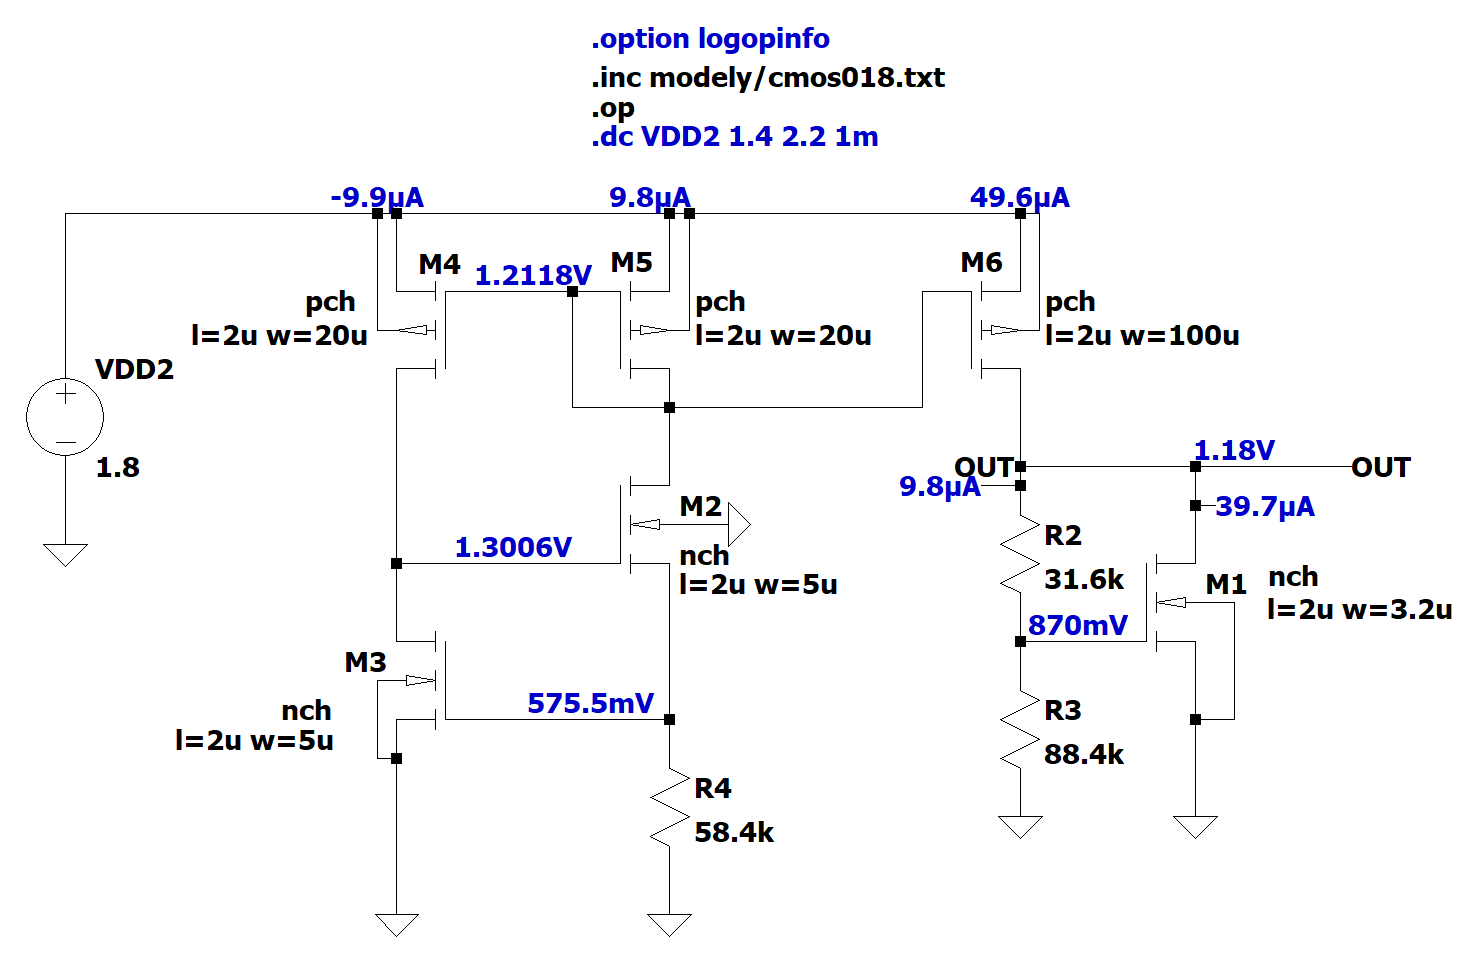
\includegraphics[width=0.9\textwidth]{text/img/LNR-op-sch.png}
    \caption{\label{fig:LNR-op-sch} Zobrazení napětí a proudu ve schématu}
\end{figure}

\vspace{10mm}
\begin{figure}[h!]
    \centering
    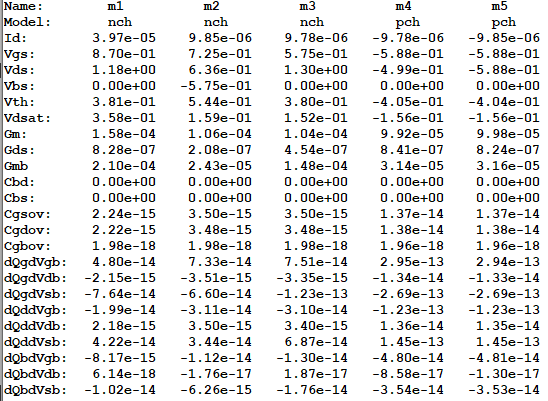
\includegraphics[width=0.9\textwidth]{text/img/LNR-op-ol.png}
    \caption{\label{fig:LNR-op-ol} Pracovní bod tranzistoru}
\end{figure}

\begin{figure}[h!]
    \centering
    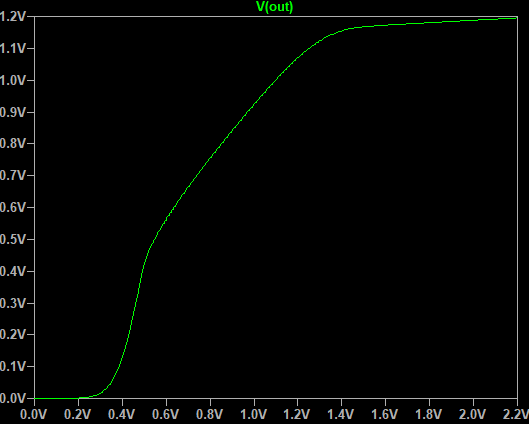
\includegraphics[width=0.9\textwidth]{text/img/LPR_zavislost.png}
    \caption{\label{fig:LNR-zav} Zobrazení napětí a proudu ve schématu}
\end{figure}

\vspace{10mm}
\begin{figure}[h!]
    \centering
    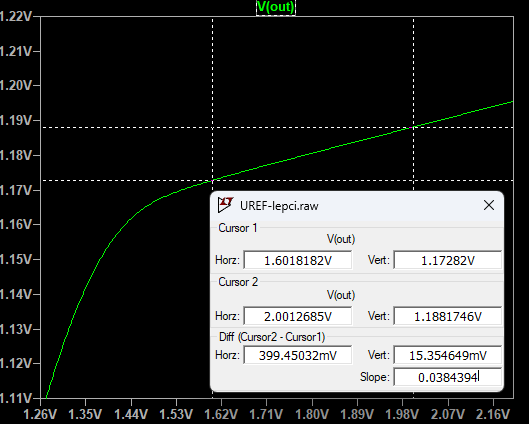
\includegraphics[width=0.9\textwidth]{text/img/LPR-detail_zavislosti.png}
    \caption{\label{fig:LNR-det-zav} Pracovní bod tranzistoru}
\end{figure}


  \newpage

% \section{Závěr}
%   Porovnání obou verzí zesilovače.

\begin{table}[h]
    \centering
    \begin{tabular}{|l|c|c|c|}
        \hline
        \textbf{Typ zátěže} & \textbf{Zesílení \(A_{U0} [-]\)} & \textbf{Rychlost přeběhu  \(SR_{fell} [V/\mu s]\)} & \textbf{šířka pásma \(GBW [MHz]\)} \\ \hline
        Odporová            & 19                               & 3.5                                                & 8.43                               \\ \hline
        Aktivní             & 38                               & 5.0                                                & 8.12                               \\ \hline
    \end{tabular}
    \caption{Porovnání obou typů zátěže}
    \label{tab:zrcadla}
\end{table}

% \clearpage
% \section*{Reference}
% \printbibliography[heading=none]

\end{document}